%%%%%%%%%%%%%%%%%%%%%%%%%%%%%%%%%%%%%%%%%%%%%%%%%%%%%%%%%%%%%%%%%%%%%%%%%%%%%%%
% krzywe i długość krzywej (reparametryzacja)
%%%%%%%%%%%%%%%%%%%%%%%%%%%%%%%%%%%%%%%%%%%%%%%%%%%%%%%%%%%%%%%%%%%%%%%%%%%%%%%
\subsection{Krzywe w czasoprzestrzeni.}
W tej części wprowadzimy pojęcie krzywej w czasoprzestrzeni. 
Jest to bardzo ważny obiekt matematyczny, gdyż służy do definiowania
wektora stycznego na rozmaitości różniczkowej~\cite{ganca1987}.
%Większość ówczesnej fizyki formuuje się w postaci wariacyjnej,
%gdzie całkowanie odbywa się po pewnej krzywej.
\begin{definition}
Krzywą sparametryzowaną (lub parametryzacją krzywej) nazywamy 
odwzorowanie 
% gładki homeomorfizm
% homeomorfizm
$ y_1 : I \ni \tau \to y_1(\tau) \in M$ klasy $c^\infty$, 
gdzie $I \subset R$ 
jest przedziałem otwartym (niekoniecznie skończonym).
\end{definition}
\begin{definition}
Parametrem dla krzywej sparametryzowanej $y_1$ 
nazywamy funkcję $ \tau_1: y_1(I) \ni p 
\to \tau_1(p) = y_1^{-1}( p )\in I$. 
Będziemy pisać
$\tau_1$ zamiast $\tau_1(p)$, wszędzie gdzie punkt $p$ 
wynika z kontekstu.
\end{definition}
\begin{definition}
Niech $y_1: I \to M$ i $y_2:J\to M$ będą parametryzacjami.
Reparametryzacją krzywej będziemy nazywać dyfeomorfizm $f : I \to J$
klasy $C^\infty$
taki, że $y_1 = y_2 \circ f$.
\end{definition}
Jeśli dla dwóch parametryzacji istnieje reparametryzacja to 
mówimy, że są one równoważne. Można łatwo pokazać, że jest to
relacja równoważności. Możliwość różnego parametryzowania tej 
samej krzywej możemy rozumieć tak, że możemy podróżować wzdłuż
krzywej w różny sposób.
\begin{definition}
Krzywą (lub krzywą niesparametryzowaną) nazywamy klasę równoważności
parametryzacji ze względu powyższą relację równoważności.
Jeżeli $y$ jest krzywą, $y_1$ jej parametryzacją z parametrem $\tau_1$
to wprowadzamy oznaczenie $y_1 =: y(\tau_1)$.
\end{definition}
\begin{figure}
\centering
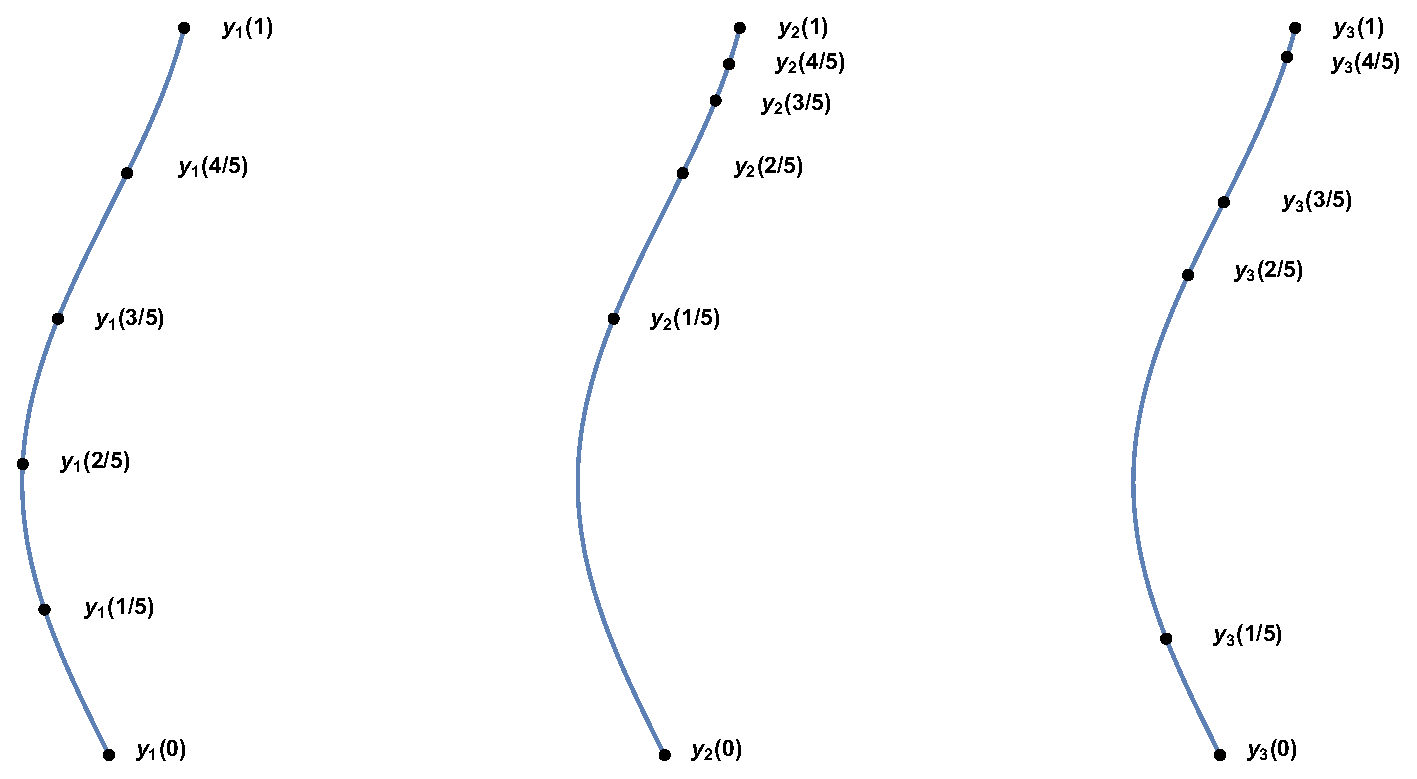
\includegraphics[scale=0.6]{curves.eps}
\caption{Różne parametryzacje krzywej $y$.}
\end{figure}
\begin{definition}
Niech $(U,\xi)$ będzie mapą w $M$ oraz $p\in U$. W tej mapie 
przez $y^\mu$ oznaczamy współrzędne krzywej $y$.
Wektorem stycznym do krzywej $y$ w punkcie $p$  
(lub wektorem prędkości w 
parametrze $\tau$) nazywamy wektor $y'(\tau)$ taki, że
\begin{align*}
%y' (\tau )= \frac{\d (\xi \circ y_1 )(\tau)
% }{\d \tau}\big|_{\tau(p)}
y' (\tau )= \frac{\d y_1^\mu }{\d \tau}
\end{align*}
Mając mapę w punkcie $p$ możemy określić bazę w danym punkcie
za pomocą wektorów stycznych do linii układu współrzędnych.
Taką bazę należy rozumieć jako bazę lokalną (bazę w punkcie $p$).
W bazie ortonormalnej macierz tensora metrycznego
przybiera postać 
\begin{align*}
( g_{\mu\nu} ) = \left(
\begin{array}{cccc}
1 & 0 & 0 & 0\\
0 & -1 & 0 & 0 \\
0 & 0 & -1 & 0 \\
0 & 0 & 0 & -1 
\end{array}
\right)
\end{align*}
Tensor metryczny określa następujący podział wektorów
\begin{align*}
g_{\mu\nu}u^\mu u^\nu > 0& \implies u \text{ - wektor czasowy}\\
g_{\mu\nu}u^\mu u^\nu = 0& \implies u \text{ - wektor zerowy}\\
g_{\mu\nu}u^\mu u^\nu < 0& \implies u \text{ - wektor przestrzenny}
\end{align*}
\end{definition}
Podział wektorów wprowadzony przez tensor metryczny $g$ 
wyróżnia trzy rodzaje krzywych. 
\begin{definition}
Krzywą $y$ nazywamy krzywą czasową (zerową, przestrzenną)
jeżeli w każdym punkcie $p \in y$ wektor $y'$ jest 
wektorem czasowym
(zerowym, przestrzennym). Linią świata cząstki
jest krzywa czasowa. 
\end{definition}
Długość $S(y(\tau))$ krzywej czasowej $y$ liczymy 
korzystając z tensora metrycznego $g$. 
Kwadrat długości elementu liniowego wyraża się przez
\begin{align*}
\d s^2 = g_{\mu\nu} \d x^\mu \d x^\nu.
\end{align*}
Stąd długość krzywej liczymy wzorem
\begin{align}\label{dlugosc_krzywej}
S( y(\tau) ) = \int_{\tau(p_0)}^{\tau(p_1)} \sqrt{g (
y' (\tau), y' (\tau) )} \d \tau.
\end{align}
Oczywiście 
długość krzywej nie powinna zależeć od wyboru parametryzacji.
Istotnie, długość dana wzorem~\eqref{dlugosc_krzywej}
jest niezmiennicza ze względu na reparametryzację.
Niech $\tau_1,\ \tau_2$ będą parametrami powiązanymi 
reparametryzacją $\tau_2 = f(\tau_1)$, taką że 
$f'(\tau_1) > 0$ (gdy $f'(\tau_1) <0$ rozumowanie 
przebiega analogicznie).
Wtedy stosując zmianę zmiennych całkowania dostajemy
\begin{align*}
S(y(\tau_2)) = 
\int_{\tau_2(p_0)}^{\tau_2(p_1)} \sqrt{g (
y' (\tau_2), y' (\tau_2) )} \d \tau_2  = 
\int_{\tau_1(p_0)}^{\tau_1(p_1)} \sqrt{g \left(
\frac{ y' (\tau_1) }{ f'(\tau_1)}, 
\frac{ y' (\tau_1) }{ f'(\tau_1)} \right)} 
f'(\tau_1) \d \tau_1  = 
\int_{\tau_1(p_0)}^{\tau_1(p_1)} \sqrt{g (
y' (\tau_1), y' (\tau_1)  )} \d \tau_1  
=S(y(\tau_1)).
\end{align*}
Stosując ten sam wzór do krzywej zerowej otrzymujemy zerową
długość.

